%% Package and Class "uiucthesis2014" for use with LaTeX2e.
\documentclass[edeposit,fullpage]{uiucthesis2018}


\usepackage[acronym,toc]{glossaries}
\newacronym{cta}{CTA}{Chicago Transit Authority}
\newacronym{usa}{USA}{United States of America}
\newacronym{ceja}{CEJA}{Climate and Equitable Jobs Act}
\newacronym{padd}{PADD}{Petroleum Administration for Defense District}
\newacronym{smr}{SMR}{Steam Methane Reformation}
\newacronym{hds}{HDS}{hydrodesulfurization}
\newacronym{esom}{ESOM}{Energy System Optimization Model}
\newacronym{hgl}{HGL}{hydrocarbon gas liquids}
\newacronym{btu}{Btu}{British thermal unit}
\newacronym{eia}{EIA}{U.S. Energy Information Administration}
\newacronym{swu}{SWU}{separative work units}
\newacronym{triso}{TRISO}{TRi-structural ISOtropic}
\newacronym{uf}{UF}{Used Fuel}
\newacronym{nfc}{NFC}{nuclear fuel cycle}
\newacronym{lwr}{LWR}{Light Water Reactor}
\newacronym{ipyc}{IPyC}{Inner PyroCarbon layer}
\newacronym{opyc}{OPyC}{Outer PyroCarbon layer}
\newacronym{htgr}{HTGR}{High-Temperature Gas-cooled Reactor}
\newacronym{uk}{UK}{United Kingdom}
\newacronym{fb-cvd}{FB-CVD}{Fluidized-Bed Chemical Vapor Deposition system}
\newacronym{bwxt}{BWXT}{BWX Technologies, Inc.}
\newacronym{usnc}{USNC}{Ultra Safe Nuclear Corporation}
\newacronym{nrc}{NRC}{U.S. Nuclear Regulatory Commission}
\newacronym{pfm}{PFM}{the Pilot Fuel Manufacturing facility}
\newacronym{tf3}{TF3}{the TRISO-X Fuel Fabrication Facility}
\newacronym{wna}{WNA}{the World Nuclear Association}
\newacronym{bwr}{BWR}{Boiling Water Reactor}
\newacronym{pwr}{PWR}{Pressurized Water Reactor}
\newacronym{hwr}{HWR}{Heavy Water Reactor}
\newacronym{gcr}{GCR}{Gas Cooled Reactor}
\newacronym{msr}{MSR}{Molten Salt Reactor}
\newacronym{lmfbr}{LMFBR}{Liquid Metal Fast Breeder Reactor}
\newacronym{rmbk}{RMBK}{graphite-moderated water-cooled reactor}
\newacronym{tru}{TRU}{transuranic isotopes}
\newacronym{mox}{MOX}{mixed oxide fuel}
\newacronym{leup}{LEU$^+$}{low enriched uranium$^+$}
\newacronym{haleu}{HALEU}{high assay low enriched uranium}
\newacronym{dre}{DRE}{Dynamic Resource Exchange}
\newacronym{ever}{EVER}{Enrichment Versatile non-Equilibrium Reactor}
\newacronym{clover}{CLOVER}{Core LOading versatile non-Equilibrium Reactor}
\newacronym{doe}{DOE}{U.S. Department of Energy}
\newacronym{pris}{PRIS}{Power Reactor Information System}
\newacronym{iaea}{IAEA}{International Atomic Energy Agency}
\newacronym{arfc}{ARFC}{Advanced Reactors and Fuel Cycles}
\newacronym{ercot}{ERCOT}{Electric Reliability Council of Texas}
\newacronym{esm}{ESM}{Energy System Model}
\newacronym{iea}{IEA}{International Energy Agency}
\newacronym{iiasa}{IIASA}{International Institute for Applied Systems Analysis}
\newacronym{bau}{BAU}{Business-as-Usual}
\newacronym{leu}{LEU}{low enriched uranium}
\newacronym{heu}{HEU}{highly enriched uranium}
\newacronym{nea}{NEA}{Nuclear Energy Agency}
\newacronym{fbcvd}{FB-CVD}{fluidized-bed chemical vapor deposition system}
\newacronym{aec}{AEC}{Atomic Energy Commission}
\newacronym{mmr}{MMR}{Micro Modular Reactor}
\newacronym{fhr}{FHR}{Fluoride Salt-Cooled, High Temperature Reactor}
\newacronym{lace}{LACE}{Los Alamos Criticality Engine}

\usepackage{xspace}
\usepackage{graphics}
\newcommand{\cycamore}{\textsc{Cycamore}\xspace}
\newcommand{\cyclus}{\textsc{Cyclus}\xspace}


\usepackage[section]{placeins}
\usepackage{booktabs} % nice rules (thick lines) for tables
\usepackage{microtype} % improves typography for PDF

\usepackage[hyphens]{url}
\usepackage{hyperref}
\usepackage{subfig}
\usepackage{hhline}
\usepackage{amsmath}
\usepackage{color}
\usepackage{multirow}
\usepackage{siunitx}
\sisetup{
    input-decimal-markers = .,input-ignore = {,},table-number-alignment = right,
    group-separator={,}, group-four-digits = true
}
\usepackage{fourier}
\usepackage{booktabs}
\newcommand\tab[1][1cm]{\hspace*{#1}}

\usepackage{threeparttable, tablefootnote}

%tikzpicture fit to page width
\usepackage{environ}
\makeatletter
\newsavebox{\measure@tikzpicture}
\NewEnviron{scaletikzpicturetowidth}[1]{%
  \def\tikz@width{#1}%
  \def\tikzscale{1}\begin{lrbox}{\measure@tikzpicture}%
  \BODY
  \end{lrbox}
  \pgfmathparse{#1/\wd\measure@tikzpicture}%
  \edef\tikzscale{\pgfmathresult}%
  \BODY
}

\usepackage{tabularx}
\newcolumntype{b}{>{\hsize=1.0\hsize}X}
\newcolumntype{q}{>{\hsize=0.5\hsize}X}
\newcolumntype{R}{>{\raggedleft\arraybackslash\hsize=0.5\hsize}X}
\newcolumntype{z}{>{\hsize=0.75\hsize}X}
\newcolumntype{s}{>{\hsize=.5\hsize}X}
\newcolumntype{m}{>{\hsize=.75\hsize}X}

\usepackage{cleveref}
\usepackage{datatool}
\usepackage[numbers]{natbib}
\usepackage{notoccite}


\usepackage{tikz}
\usetikzlibrary{positioning, arrows, decorations, shapes}

\usetikzlibrary{shapes.geometric,arrows}
\tikzstyle{process} = [rectangle, rounded corners, minimum width=2.5cm, minimum height=1cm,text centered, draw=black, fill=blue!30]

\tikzstyle{object} = [ellipse, rounded corners, minimum width=3cm, minimum height=1cm,text centered, draw=black, fill=green!30]
\tikzstyle{objectr} = [ellipse, rounded corners, minimum width=3cm, minimum height=1cm,text centered, draw=black, fill=red!30]

\tikzstyle{empty} =  [rectangle, rounded corners, minimum width=2.5cm, minimum height=0.7cm,text centered, draw=black, fill=white!30]
\tikzstyle{arrow} = [thick,->,>=stealth]

\tikzstyle{decision} = [diamond, draw, fill=blue!20,
text width=6em, text badly centered, node distance=3cm, inner sep=0pt]
\tikzstyle{block} = [rectangle, draw, fill=blue!20,
text width=9em, text centered, rounded corners, minimum height=4em]
\tikzstyle{block2} = [rectangle, draw, fill=yellow!20,
text width=9em, text centered, rounded corners, minimum height=4em]
\tikzstyle{line} = [draw, -latex']
\tikzstyle{cloud} = [draw, ellipse,fill=red!20, node distance=3cm,
minimum height=4em]


\title{Optimizing TRISO Reactor Fuel Enrichment and Cyclus Memory Efficiency}
\author{Nathan Sean Ryan}
\department{Nuclear, Plasma, Radiological Engineering}
\schools{B.S., University of Illinois - Urbana Champaign, 2022}
\msthesis
\advisor{Madicken Munk}
\degreeyear{2024}
\committee{Assistant Professor Madicken Munk \\ Professor Kathryn D. Huff}

\begin{document}
\maketitle

\frontmatter
%% Create an abstract that can also be used for the ProQuest abstract.
%% Note that ProQuest truncates their abstracts at 350 words.
\begin{abstract}

%% Create an abstract that can also be used for the ProQuest abstract.
%% Note that ProQuest truncates their abstracts at 350 words.
This is the abstract.

\end{abstract}

\chapter*{Acknowledgments}

I would like to thank Prof. Madicken Munk, who mentored me as a student and who
constantly inspires me to think big and find the impact in my work. Relatedly,
I would like to thank Prof. Kathryn Huff, who has been a mentor to me at every
step of my collegiate education and who shows me how to be a happy warrior.

I want to thank my fellow graduate students and the members of
\gls{arfc}; particularly Dr. Amanda Bachmann, Sam Dotson, Nataly Panczyk, Olek
Yardas, Zo\"{e} Richter, Dr. Gwendolyn Chee, Dr. Sun Myung Park, Rhys
MacMillian, and Ceser Zambrano. I would like to especially thank Luke Seifert
for his assistance in running the Serpent simulations in this work.

Throughout the years, I have learned much from my group mates, advisors, and
mentors, but I would be remiss not to acknowledge that I went to the school of
open source and learned much from countless developers who work openly to
better science. Particularly the \cyclus community, especially Prof. Paul P.H.
Wilson, Dr. Katie Mummah, Jin Whan Bae, and Dr. Eva Davidson.

I owe many thanks to my parents, brother, grandparents, family, partner, and
friends who have reminded me---sometimes to my chagrin---that life keeps going
outside the walls of my office. To my cousin Matthew, I can not wait to explain
this part of my life to you someday when we are reunited because I know you
will have questions.

This research was performed, in part, using funding received from the DOE
Office of Nuclear Energy's Nuclear Energy University Program (Project 23-29656
DE-NE0009390) 'Illuminating Emerging Supply Chain and Waste Management
Challenges'.

This research was supported in part by an appointment to the Oak Ridge National
Laboratory Research Student Internships Program, sponsored by the U.S.
Department of Energy and administered by the Oak Ridge Institute for Science
and Education.

%% The thesis format requires the Table of Contents to come
%% before any other major sections, all of these sections after
%% the Table of Contents must be listed therein (i.e., use \chapter,
%% not \chapter*).  Common sections to have between the Table of
%% Contents and the main text are:
%%
%% List of Tables
%% List of Figures
%% List Symbols and/or Abbreviations
%% etc.

\tableofcontents
\listoftables
\listoffigures

%% Create a List of Abbreviations. The left column
%% is 1 inch wide and left-justified
%\chapter{List of Abbreviations}
%\printglossaries
%% Create a List of Symbols. The left column
%% is 0.7 inch wide and centered

\pagebreak
\mainmatter

\chapter{Introduction}
\label{ch:introduction}

Introduction \cite{huff_extensions_2014}.

% The United States contributed more than $12.5\%$ to the total carbon emissions
in 2020 \cite{european_commission_joint_research_centre_ghg_2021}. In response
to growing climate concerns local, state, and national governmental bodies have
announced myriad supports for clean energy projects; however, when you add
lenses of environmental justice and life cycle analysis, these transitions might
result in displacement instead. In 2012 Richard York from the Oregon State
Department of Sociology and Environmental Studies published a study of the
50-year history of alternative-energy installations to our modern grid
asserting that "to displace 1 kWh of fossil-fuel electricity requires
generating more than 11 kWh of non-fossil-fuel electricity,"
\cite{york_alternative_2012}. This conversion was based on 6 models of fossil
fuel use from 1960-2009, accounting for levels of urbanization, manufacturing,
age, and a variety of energy technologies.

This result challenges the assumption that there is a one-to-one relationship
between energy facilities with comparable power. In 2019 York and co-author
Shannon Bell further developed this idea saying that such proportional
representation studies "do not focus their discussions on or graphically
present the absolute quantity of energy in their assessments of purported
energy transitions," \cite{york_energy_2019}. They demonstrate with Figure
\ref{fig:percent_total_energy} that the proportional representation misses that
the total demand for energy has dramatically increased since the Industrial
Revolution. What may have looked like a transition in the mid-1800s from
biofuels to coal is merely a displacement, and they show that the energy
consumption of biofuel has increased since the early 1900s.

\begin{figure}[H]
  \subfloat[Proportional Energy Use.\label{fig:percent}]{%
    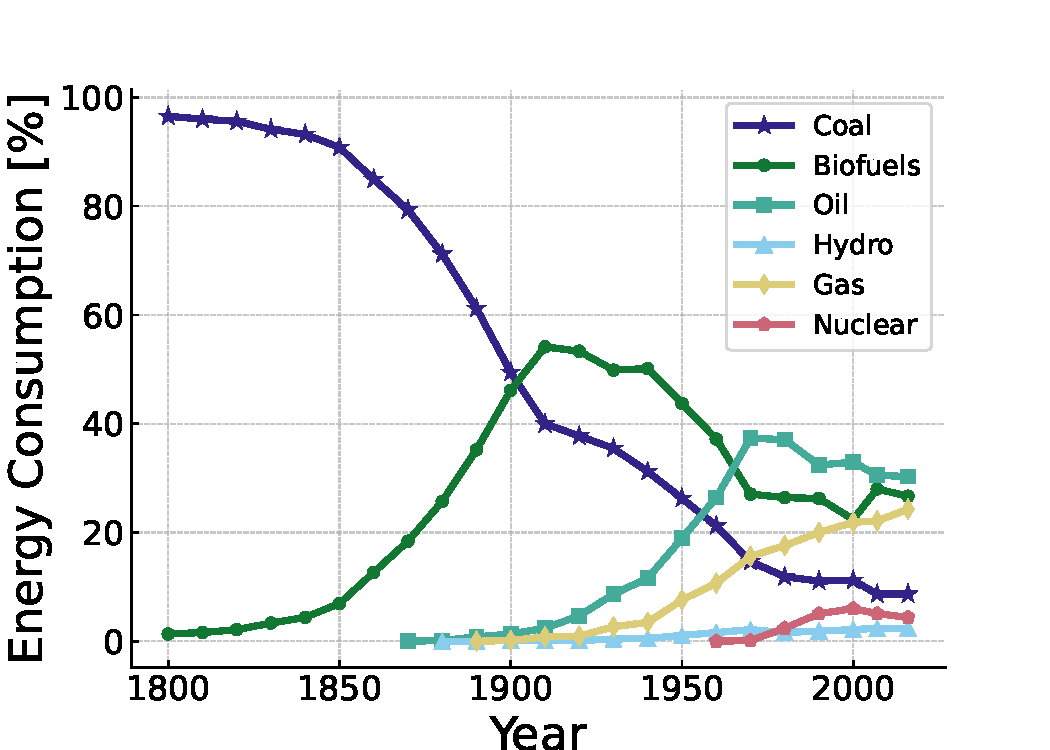
\includegraphics[width=0.499\textwidth]{images/leg_frame/proportional_fuel_use.pdf}
 }
  \hfill
  \subfloat[Total Energy Use.\label{fig:total}]{%
    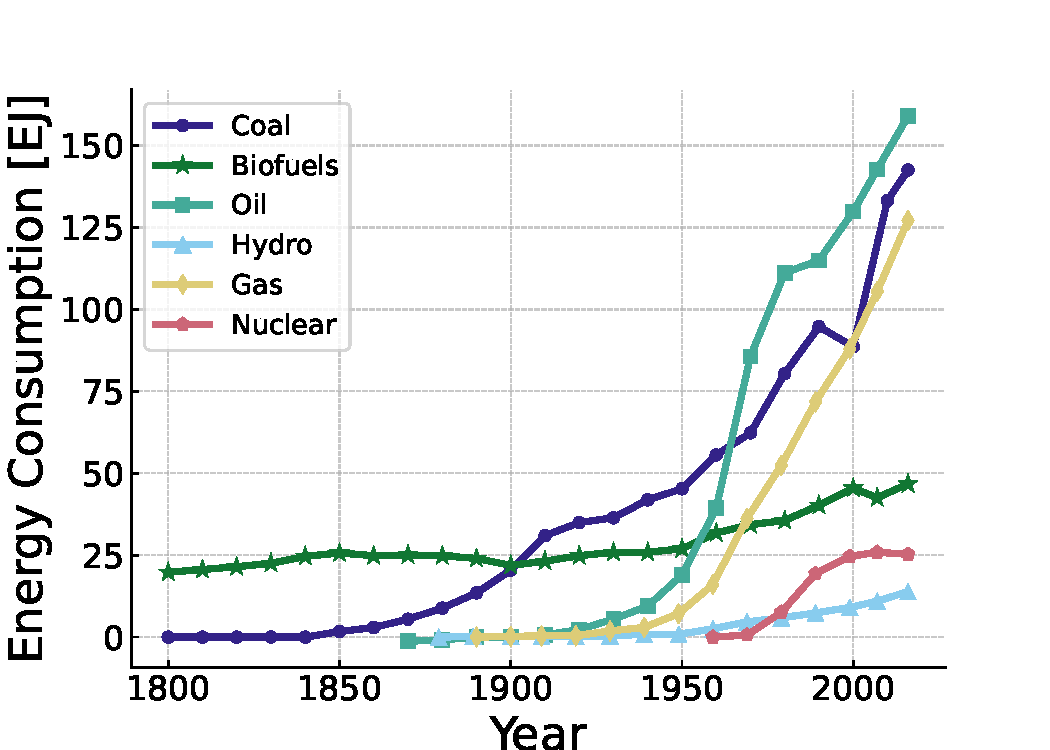
\includegraphics[width=0.499\textwidth]{images/leg_frame/total_fuel_use.pdf}
 }
  \caption{
    Global energy consumption (exajoules) by source. 1800--2017
    \cite{york_energy_2019}.}
  \label{fig:percent_total_energy}
\end{figure}

Similarly, what looks in Figure \ref{fig:percent} like a transition away from
coal in the early 1900s, with the introduction of alternatives like oil and
hydroelectricity, belies the continued increase in coal consumption into the
early 2000s. If what we have axiomatically understood as a transition is not
happening, we arrive at the kernel of several grand challenges to our society
and our elected officials. The semantic difference between a transition and a
displacement is not the core concern, instead we must focus on realistically
presenting the increasing energy needs of our society.

The policy inertia behind the monetary valuation of our energy system is
something that future generations could overcome, upending the incentives
policymakers might implement to drive an actual transition instead of a
displacement as we have discussed. If decision-makers focus on what a policy
will do only for the term of their service, they drastically undervalue the
impact that daily climate actions will have hundreds of years down the line. We
see this dichotomy in the 2020 grid failings in Texas during the unseasonably
cold front they experienced. From the outside, we can see how an extreme
weather event would create a great demand. This case is a microcosm of a
drastic change in the values a society had in an energy grid. In the span of a
couple of weeks a state that had proudly touted its achievement of a sustained
grid \cite{texas_ercot_nodate} experienced massive failures only for its
service to resume.

Since 2020, the \gls{ercot} has been working to update its grid to be more
resilient to such events, the Grid Deployment Office of \gls{doe} published a
report in 2024 outlining the more than \$270 billion of savings from increasing
connections to the Texas Interconnection
\cite{doe_transmission_planning_study_2024}. Concurrent with this announcement,
the \gls{doe} announced \$1.5 billion transmission investment that would go to
four projects in Texas, New Mexico, Louisiana, Mississippi, Maine, Oklahoma,
and Arizona \cite{doe_tran_announce_2024}. These projects are expected to be
completed by 2026 and will increase the capacity of the grid by 1.5 GW. This is
a step in the right direction, but it is not enough to ensure that the grid
will be resilient to future extreme weather events.

We can legislate for such changes by developing policy frameworks that bring in
the community and address our changing values for energy systems. Elisa Papadis and George Tsatsaronis set out to update the vision for a well-designed policy package in their 2020 paper, surmising that producing policy "with measures such as carefully introduced targeted investment subsidies, performance standards and mandates, communication and education campaigns and a CO$_2$ tax for global aviation and shipping" constitutes achieving this legislative framework \cite{papadis_challenges_2020}. This approach will require geographically bespoke solutions that draw in stakeholders, and focus on serving the needs of the future stakeholders as well as the current ones. They go on to advocate for expansion and investment in the massively complex \gls{usa} power grid due to the requirements of more flexibly generated capacity.

Flexibility is a seemingly ubiquitous goal of decarbonized industries, like
chemical producers, which highlight big emitters that are large volume/
low-profit goods (disincentivizing development)
\cite{mallapragada_decarbonization_2023} or farm researchers who highlight the
growing importance of human intervention as climate change impacts their crop
in a negative feedback cycle \cite{farokhi_soofi_farm_2022}. The start is
focusing our efforts where investment can have the largest impact in the
shortest time, and to consult the changing valuation of stakeholders in how we
deploy electrification and updates to the grid.

\chapter{Background}
\label{background}
\section{The Nuclear Fuel Cycle}


In the US, we keep each of these facilities separate in the front-end of
the fuel cycle in a "collect and wait" pathway \cite{cycle_risks}. In
lieu of a long or interim solution for the \gls{uf}, the back end of the
\gls{nfc} is collocated with the reactors that burn the fuel (with the
minor exception of the consolidated storage facility in Morris Illinois).

Nuclear fuel has the capacity to be
reprocessed and recycled into a different fuel type that can produce
usable power for several cycles, called a "closed" fuel cycle.





 \begin{figure}[h]
    \centering
    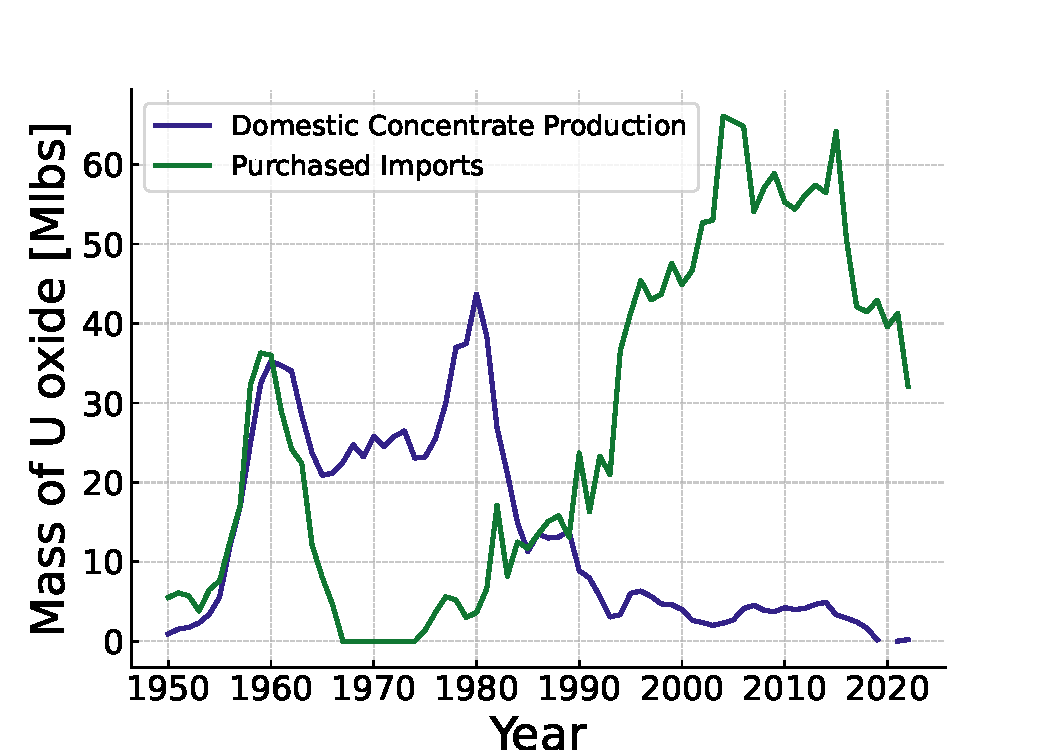
\includegraphics[scale=0.8]{images/intro/uranium_production_imports.pdf}
    \caption{Foregin and domestic uranium purchases over time \cite{eia_monthly_energy_review_2024}.}
    \label{fig:foregin_u3o8}
 \end{figure}

\section{Transition Scenarios}
% Provide an introduction to the literature review. Explain the scope of the
% review.

\section{Theoretical Background}
% Discuss the theoretical framework and key concepts that underpin the research.

% Talk about the value and purpose of energy system modeling.

\section{Nuclear Fuel Cycle Simulation}
Review the literature related to NFC sims.

\section{Non Equilibrium Fuel Cycles}
Review the literature related to noneq NFC.

\section{Memory Efficiency}
Review the literature related to the third subtopic. Summarize key findings and highlight important studies.

\section{Gaps in the Literature}
Identify gaps or limitations in the existing literature. Discuss areas where further research is needed.

\section{Summary}
Provide a summary of the key points discussed in the literature review. Highlight the relevance of the reviewed literature to your research.


\section{TRISO Fuel}
\section{TRISO Fuel}
\label{sec:triso_fuel}

In this work, we adapt the approach of Bachmann et al.
\cite{bachmann_enrichment_2021} to focus on \gls{triso} fueled reactor designs
alongside traditional fuel forms at various enrichments. \gls{triso} is not a
classification of enrichment; several reactor designs use different fuel
enrichments that are all \gls{triso}. Here we will distinguish the
production of \gls{triso} from the traditional metallic fuels used in
\glspl{lwr} outlined in Section \ref{sec:nfc}.

Coating the fuel particles is a critical step in the fabrication of \gls{triso}
fuel, and the idea has existed in nuclear fuel design spaces since the 1950s
\cite{price_dragon_2012} with the Dragon project. In 1957, the Harwell facility
began coating spherical fuel particles, and in 1961, researchers modified the
particle coating to include a silicon carbide layer to trap cesium, strontium,
and barium--which diffused through the single pyrolytic carbon layer.
Concurrently, in 1958, a report to the \gls{aec} introduced the concept of a
pebble bed pile (first proposed by Daniels
\cite{f_b_daniels_suggestions_1944}) to the broader nuclear community.
Researchers in Germany, China, and the UK have proposed, built, and operated
similar designs since then, with companies in the \gls{usa} looking to deploy
modern versions of the technology.

In a 2019 paper, authors Demkowicz, Liu, and Hunn \cite{particle_review_2019}
authors describe the fuel as a particle encapsulated in layers of pyrolytic
carbon and silicon carbide; a \gls{fbcvd} applies each of these layers. As
shown in Figure \ref{fig:triso_layers}, the layers are frequently ordered with
a fuel kernel at the center, followed by layers of porous carbon buffer, inner
pyrolytic carbon, silicon carbide, and outer pyrolytic carbon. The fuel kernel
is typically composed of uranium dioxide, and it is surrounded by a porous
carbon buffer using acetylene in the \gls{fbcvd} as it has a relatively low
density. The silicon carbide layer encapsulates the pyrolytic carbon layers and
provides a barrier to fission products. A mix of methyltrichlorosilane and
hydrogen is sufficient for SiC deposition without argon. The inner and outer
pyrolytic carbon layers isolate the silicon carbide layer and provide a barrier
to the coolant; the \gls{fbcvd} applies these layers using a mix of propylene,
acetylene, and argon.

\begin{figure}[H]
    \centering
    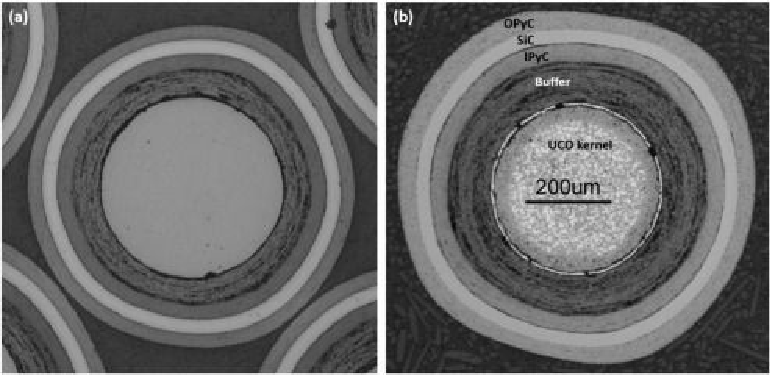
\includegraphics[scale=0.98]{images/triso_review/triso_layers.pdf}
    \caption{TRISO Fuel Particle Layers \cite{particle_review_2019}}
    \label{fig:triso_layers}
\end{figure}

Through a heat and pressure setting process, fabricators create a fuel matrix
that accepts the coated particles. These matrices hold the \gls{triso}
particles in graphite and carbonized resin and are set under heat and pressure,
often overcoated to prevent particle-particle interactions. The resulting fuel
type is incredibly robust and can reduce proliferation concerns due to the
difficulty separating the particles from the matrix and the fuel from the
particles. The fuel can withstand high temperatures and burnups, which can be
advantageous in reactor designs that require high temperatures for efficient
operation.

\section{Metrics}
\label{sec:metrics}

% discuss the metrics you are using
In this work, we will develop a model of nuclear energy in the \gls{usa} using concepts from \glspl{esm} on scenarios that compare the transition from our current fleet to incorporate advanced reactor technologies not currently deployed. To compare these scenarios, we have chosen to focus on a few key metrics: \gls{swu}, energy output, mass of fuel, and reactor deployment.

\subsection{Separative Work Units}
\label{sec:swu}
% justify what swu is and why it is a valuable metric
The process of enriching uranium is a critical step in the nuclear fuel cycle, and, as we have highlighted, is expected to be a bottle neck in the deployment of advanced reactors. \gls{swu}, or a Separative Work Unit, is a ubiquitous measure of effort that goes into producing nuclear fuel. It is simplified as:
\begin{align}
    SWU&= (P \times V(x_p) + T \times V(x_t) - F \times V(x_f))\times t\nonumber
    V(x_i)&= (2 * x_i - 1) \times \ln\left(\frac{x_i}{1 - x_i}\right)\nonumber
    \intertext{Where:}
    SWU&= \mbox{Separative Work Units [kgSWU]}\nonumber\\
    P&= \mbox{Product mass flow rate [kg/d]}\nonumber\\
    F&= \mbox{Feed mass flow rate [kg/d]}\nonumber\\
    T&= \mbox{Tails mass flow rate [kg/d]}\nonumber\\
    V&= \mbox{Separation Potential [-]}\nonumber\\
    x_i&= \mbox{Weight fraction of $^{235}U$ in the i stream [-]}\nonumber\\
    x_p&= \mbox{Weight fraction of $^{235}U$ in the product stream [-]}\nonumber\\
    x_f&= \mbox{Weight fraction of $^{235}U$ in the feed stream [-]}\nonumber\\
    x_t&= \mbox{Weight fraction of $^{235}U$ in the tails stream [-]}\nonumber\\
    t&= \mbox{Time [d]}\nonumber
\end{align}

In this work, we will compare the \gls{swu} required for each scenario to understand the relative effort required to deploy the reactors and provide a stable precursor to economic calculations. As we mention in Section \ref{sec:leup}, the definition used in the literature for \gls{leup} can be tied to the upper limit on enrichment for a Category III facility. The \gls{leup} fuel, as shown in Table \ref{tab:ar_defs}, is enriched to 9.95\% $^{235}$U, which would fall under the Category III limit. The \gls{haleu} fuel would require Category II facilities to achieve the 19.75\% $^{235}$U and 15.5\% $^{235}$U enrichment for the \gls{mmr} and \gls{xe} \gls{haleu}respectively. The \gls{swu} required for each scenario will be compared to understand the relative effort required to deploy the reactors and provide a stable precursor to economic calculations.

In Table

\begin{table}
    \centering
    \caption{SWU calculation values for each fuel type}
    \label{tab:swu_vals}
    \begin{tabular}{c c}
        \hline
        \textbf{Variable} & \textbf{Value}\\
        \hline
        \gls{mmr} \gls{leup} $x_p$ & 0.0995\\
        \gls{mmr} \gls{haleu} $x_p$ & 0.1975\\
        \gls{xe} \gls{leup} $x_p$ & 0.0995\\
        \gls{xe} \gls{haleu} $x_p$ & 0.155\\
        \gls{leu} $x_p$ & 0.045\\
        $x_f$ & 0.00711\\
        $x_t$ & 0.002\\
        \hline
    \end{tabular}
\end{table}

\subsection{Energy Output}
\label{sec:energy_output}

The deployment of reactors in this work is based on energy demand, which
approximates the complicated relationship that generators and utilities
have with power expansions. The reactors simulated herein have a static peak energy output, so the nuance in the fleet's ability to meet the demand comes from the deployment scheme and limitations in the fuel supply chain. We will devote time to discussing the realistic features of each scheme. \cyclus tracks the energy output of each reactor, and we will compare that with the demand scenarios to understand the relative performance of each deployment scheme.


\subsection{Mass of Fuel}
\label{sec:mass_of_fuel}

\cyclus tracks the mass of material in each transaction, in this work we will characterize the deployment challenge ahead of us using the fresh and used fuel accumulation to show the relative mass of fuel required to deploy the reactors in each scenario. From the mass of fuel, and knowledge of the fuel design, these results can be converted into cost metrics, transportation modeling, and hypothetical repository space considerations.

\section{\cyclus}
\section{\cyclus}
\label{sec:cyclus}
% fix that, too informal and introduces archetypes without context.
\cyclus is an agent-based \gls{nfc} simulator that is versatile, open source, and modular. The software achieves this versatility through a series of generic archetypes that are primarily transaction based. Over the years, the user community and developers have created a litany of nuclear specific archetypes for everything from proliferation assessment to fuel burnup. Many standard fuel cycle facilities have been implemented in the \cycamore repository on GitHub, which holds technology-agnostic archetypes for material sources, material sinks, enrichment services, separations capabilities, and a generic reactor.

% discuss recipes
As \cyclus is a transactions code and not necessarily a physics code,
the reactors incorporate reactor physics through pre-defined "recipes,"
where the user specifies the isotopic concentration of the fresh and
used fuel.

Users approximate the burnup of each fuel element with the
same input recipe as the same; however, in this work we incorporate a
cascading enrichment from \gls{leu+} to \gls{haleu}.
% find a citation or source that companies are actually going to do that
% (best case scenario is find it for each reactor you do it for)

% discuss EVER and CLOVER?
Novel in this work is our use of a low fidelity archetype based on the
\cycamore reactor %\cite{the summer poster}. \gls{ever}

\gls{ever} allows the user to specify multiple recipes for the fuel and
change between them at specific times.


% discuss DRE
As we have discussed, \cyclus's primary function is to keep track of
material transactions between agents. This is accomplished through the
\gls{dre}, which functions like a market where each agent brings a bid
for what and how much material they need and suppliers are matched with
buyers % cite something here.


\subsection{Archetypes and Time Management}
\label{sec:archetypes_and_time_management}

Throughout the \cyclus ecosystem, archetypes interact with the \gls{dre} and each other in a fixed, user defined, time step, forcing the entire simulation to operate on the smallest universal time step. For example, if a fabrication facility can produce material every 2 months but the enrichment facility can only provide material every 3 months, then we would need to use a 1 month time step to capture both. When the time step is smaller than the minimum for a given facility, that facility still participates in the \gls{dre} with a 0 bid. These zero bids, across hundreds of facilities, add complexity and inefficiencies to solving the transaction problem at each time step.

Examining the \cyclus ecosystem, we identified an archetype called $Pattern_Sink$ wherein the user can alter the frequency that the material sink, often called the repository, can accept material. We have created an example of this archetype in action with a simple A-B-C scenario, shown in Figure \ref{fig:a-b-c}. In this scenario, material is received from a source (A) to a reactor (B) with a final (C) sink that can only accept material at a certain frequency.

\begin{figure}
    \centering
    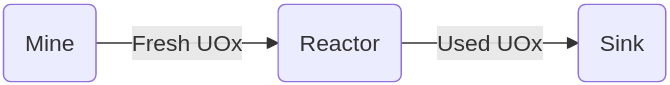
\includegraphics[scale=0.4]{images/cyclus/a-b-c.png}
    \caption{Simple A-B-C Scenario}
    \label{fig:a-b-c}
\end{figure}

If we track the material being received by the sink it becomes clear that this frequency simply alters how frequently the archetype updates its internal understanding of time. As a consequence, it appears in Figure \ref{fig:pattern_freq_50} as though multiple groups of material are received in one time step despite this archetype not having an idea of individual shipments. The way this archetype accomplishes the artificial restriction on accepting material is by simply not updating the time step that the archetype is at until the next universal time step is met. Regardless of function, this is the only example of flexibility of timestep we found in the ecosystem.

\begin{figure}
    \centering
    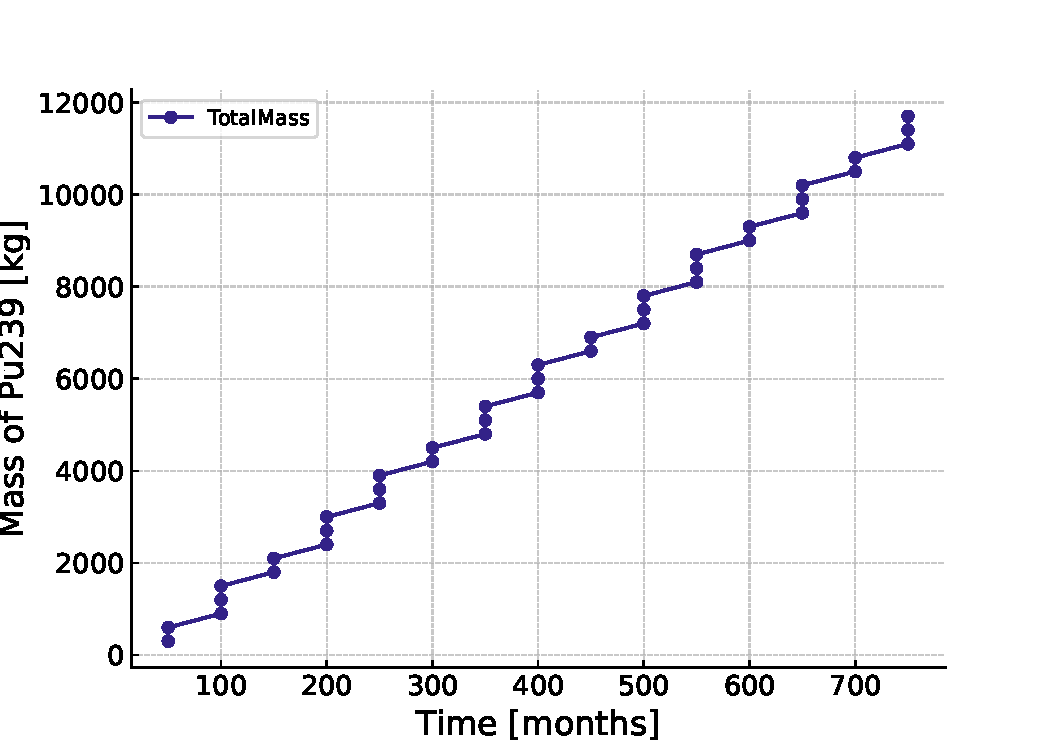
\includegraphics[scale=0.4]{images/cyclus/pattern_sink_fuel_transactions.pdf}
    \caption{Production of $^{239}$Pu with a frequency of 50 months}
    \label{fig:pattern_freq_50}
\end{figure}

In this work we implement a fundamental toolkit capability that any archetype in the Cyclus ecosystem can take advantage of with one implementation.


\chapter{Deployment Scenarios}
\label{ch:scenarios}

In this chapter, we will discuss the transition scenarios for the deployment of new nuclear reactors in the \gls{usa} and the reactor models used in this work. We will also discuss the theoretical framework and key concepts that underpin the research, and the results for each deployment scheme.

\section{Transition Scenarios}
\label{sec:transition_scenarios}
% Discuss the theoretical framework and key concepts that underpin the research.

As the energy landscape evolves, compounding
factors will drive the actual deployment of these reactors in ways this work
does not capture. The value of energy system modeling and this type of
transition scenario is to understand the implications of deployment compared
with and measured relative to business-as-usual cases with similar
approximations.

We use this chapter to explore the deployment schemes we have
implemented---outlined in Table \ref{tab:deployment_schemes}---, and the demand
growth scenarios we have considered---outlined in Table
\ref{tab:demand_scenarios}. In Appendix \ref{sec:considered_deployment_schemes}
we will discuss two additional deployment schemes that we implemented, but
have not incorporated as they are more useful for problems not considered herein.

\begin{table}[H]
    \centering
    \caption{Deployment Schemes}
    \label{tab:deployment_schemes}
    \begin{tabular}{p{0.15\linewidth} p{0.27\linewidth} p{0.50\linewidth}}
        \hline
        \textbf{Status} & \textbf{Scheme} & \textbf{Description} \\
        \hline
        \multirow{4}{*}{Incorporated} & Greedy Deployment & Deploy the largest
        reactor first at each time step, fill in the remaining capacity with
        the next smallest, and so on. \\
        & Random Deployment & Uses a date and hour as seed to sample the
        reactors list randomly. \\
        & Initially Random, Greedy Deployment & Randomly deploys reactors until
        a reactor bigger than the remaining capacity is proposed for each time step,
        then fills the remaining capacity with the greedy algorithm. \\
        % & Single Reactor & A single reactor model is deployed as the existing fleet is decommissioned.\\
        \hline
        \multirow{2}{*}{Not Incorporated} & Capped Deployment & There is a
        single-number capacity for one or more of the reactor models. \\
        & Pre-Determined Distribution Deployment & One or more reactors have a
        preset distribution, and a smaller capacity model fills in the gaps. \\
        \hline
    \end{tabular}
\end{table}

We apply these deployment schemes to demand growth scenarios based on two
predictions of future energy demand. The \gls{eia} publishes demand expansion
projections for the totality of \gls{usa} \cite{eia_aeo_2023}. The
administration has refrained from publishing AEO 2024 in light of recent
accelerations in demand growth. Our assumptions for the low-growth scenarios
are that the relative percentage of nuclear power remains constant and that the
relative performance of the various fuel cycle metrics we simulate will remain
constant. Our high-growth scenarios come from the \gls{doe} Liftoff Report
\cite{julie_liftoff_pathways_2024}, which does not reflect this constant
percentage assumption for nuclear power in their demand scenarios. Their growth
projections are specific to nuclear deployment increases and the number is
agnostic to the total increase.

\begin{table}[H]
    \centering
    \caption{Demand Growth Scenarios}
    \label{tab:demand_scenarios}
    \begin{tabular}{c c c}
        \hline
        \textbf{Demand Growth} & \textbf{Year-to-Year Increase} & \textbf{Source}\\
        \hline
        No growth & 0\% & na\\
        Low growth & 0.17\%, 0.5\%, 1\%, & \cite{eia_aeo_2023}\\
        High growth & 3.5\%, 5.6\% & \cite{julie_liftoff_pathways_2024}\\
        \hline
    \end{tabular}
\end{table}

Each growth scenario is deployed under two regimes: 1) the reactors are never
fueled with \gls{leup}; 2) the \gls{mmr} and \gls{xe} reactors are fueled with
\gls{leup} until 2040, when they move to \gls{haleu}. \glspl{mmr} deployed
before this fuel transition will continue to use \gls{leup} fuel until the end
of their lifetime as they do not refuel; however, the \gls{xe} reactors will
refuel with \gls{leup} until 2040, when they will refuel with \gls{haleu}. The
AP1000 reactors will continue to use \gls{leu} fuel throughout the simulation.

Under each regime, each growth scenario is met by deploying reactors using the
schemes outlined in Table \ref{tab:deployment_schemes}. We will discuss the
results of these deployment schemes in the following sections. We will also
discuss the limitations of this work and propose future work. Regardless of the
regime, each deployment scheme will attempt to deploy reactors to meet the
capacity outlined in Figure \ref{fig:dep_goals}.

\begin{figure}[H]
    \centering
    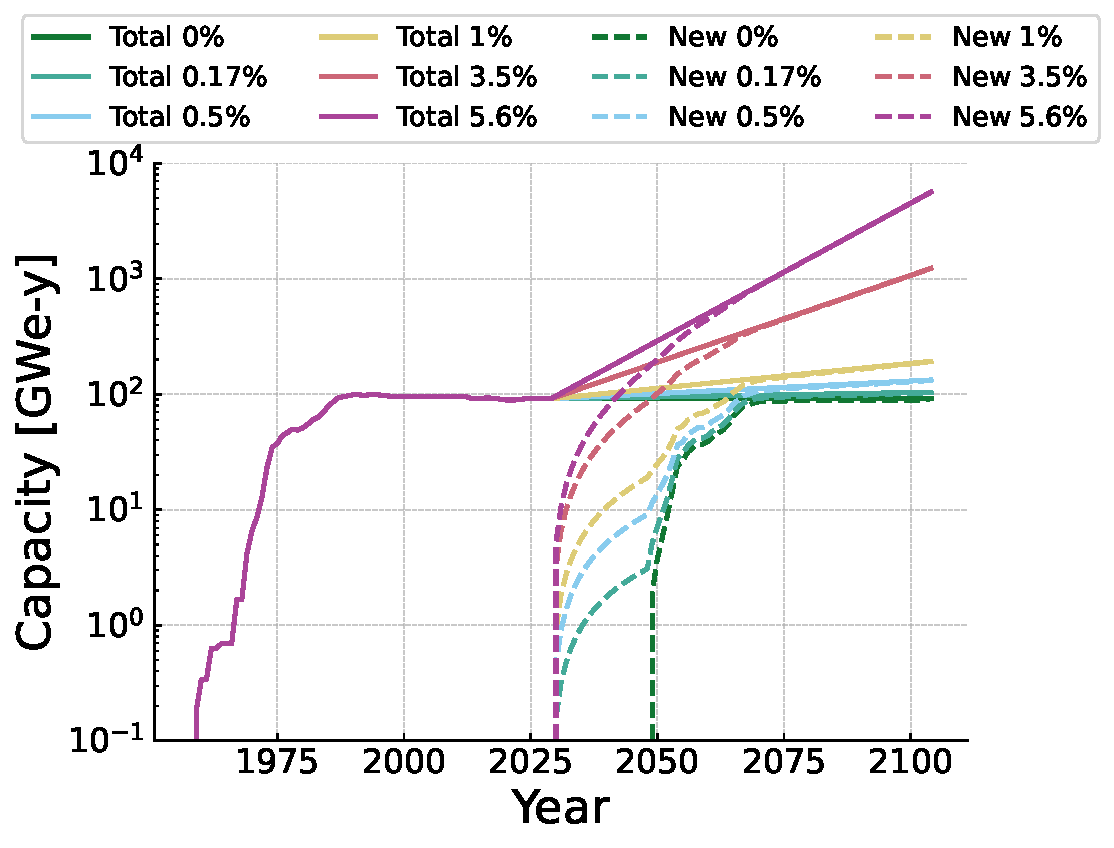
\includegraphics[scale=0.7]{images/results/deployment_calcs/total_new_capacity_scenarios.pdf}
    \caption{Total and new nuclear capacity deployed in each scenario}
    \label{fig:dep_goals}
\end{figure}

As shown, advanced reactors (for the purposes of this work the designs are the:
\gls{mmr}, \gls{xe}, and AP1000) begin deployment in 2030. While this is an
aggressive deployment schedule, \cite{bachmann_thesis_2023} established that
the precise deployment start did not significantly impact the total results for
this type of analysis and could reasonably serve as an upper bound of
deployment. The business-as-usual or, as we will refer to it, no growth
scenario does not require the deployment of a new nuclear reactor until just
before 2050, whereas the other scenarios understandably commence deployment in
2030. As we have presented the capacity on a logarithmic plot, the linear
appearance of the data belies the compounding effect that the year-to-year
percentage growth requires.

We will focus on the results of the no growth and $3.5\%$ (corresponding to a doubling of nuclear by 2050) scenarios, and the results for the other scenarios are available in Appendix \ref{ch:additional_results}.

\chapter{Memory Efficiency}
\label{ch:memory}

\chapter{Conclusions}
\label{ch:conclusions}

\section{Assumptions}
\label{sec:assumptions}

\begin{itemize}
    \item The demand increase assumes that nuclear energy's share of generation remains constant over time. When we say a 15$\%$ increase in demand, we mean a 15$\%$ increase in nuclear energy generation (as the EIA numbers are meant to reflect the total energy demand, this conversion is only possible by assuming that the percentage of nuclear capacity is the same). This assumption is not reflected in the demand scenarios from the \gls{doe} liftoff report, which are specific to nuclear deployment increases and the number is agnostic to the total increase.
    \item \gls{lwr}s have an 18 month cycle with no deviation.
    \item \gls{lwr}s have a regular 1 month outage.
    \item \gls{lwr}s have an assembly size of 427.38589211618256.
    \item \gls{lwr}s have a batch size of 80.
    \item All reactors have constant power output (when not in outage) over their lifetime.
    \item No new \gls{lwr}s are built after 2024. % not really the case anymore
    \item \gls{lwr}s have no additional outages other than the regular 1 month outage.
    \item Essentially assume that the supply chain is not a limiting factor in the deployment of new reactors, we make no requirements that it is necessarily located in the \gls{usa}, but we make no effort to explicitly realize the global nature of the supply chain.
    \item We treat the fabrication and enrichment of fuel as a black box, and do not consider the variance in time/resources/regulation required for the fuels we include.
\end{itemize}

\section{Limitations}
\label{sec:limitations}

\begin{itemize}
    \item The \gls{eia} is taking a year off in producing their report to better account for increased behind-the-meter investment, AI needs, and data center expansions \cite{eia_annual_outlook_canceled_2023}; they have indicated that these factors could be substantial.
    \item Do not directly incorporate international understanding of the supply chain.
\end{itemize}


\section{Future Work}
\label{sec:future_work}





\chapter{Appendix}
\chapter{LWRs Simulated}
\label{app:lwrs}

In this work we pull publicly available information from the \gls{pris} database to simulate the \gls{lwr} fleet in the \gls{usa}. The \gls{pris} database is a collection of information on nuclear power plants around the world, and is maintained by the \gls{iaea}. For the sake of completeness and replication of this work in Tables \ref{tab:lwr_fleet_1}, \ref{tab:lwr_fleet2}, and \ref{tab:lwr_fleet3}; we have also included the \gls{lwr} fleet that we have simulated in this work and a notebook is available on GitHub ((((((((((((cite)))))))))))) to pull the same information we used.


\begin{table}[!ht]
    \centering
    \caption{LWR Fleet Simulated, A-K}
    \label{tab:lwr_fleet_1}
    \begin{tabular}{c c c c c c c c c c}
    \hline
    \textbf{Name} & \textbf{State} & \textbf{Type} & \textbf{Vendor} & \textbf{Core size} & \textbf{Startup date} & \textbf{License} & \textbf{Retirement} & \textbf{Power cap} \\
    \hline
    Arkansas Nuclear One 1&AR & PWR & B\&W & 177 & 1974 & 2034 &      & 836.0 \\
    Arkansas Nuclear One 2&AR & PWR & CE   & 177 & 1978 & 2038 &      & 988.0 \\
    Beaver Valley 1       &PA & PWR & WE   & 157 & 1976 & 2036 &      & 908.0 \\
    Beaver Valley 2       &PA & PWR & WE   & 157 & 1987 & 2047 &      & 905.0 \\
    Big Rock Point        &MI & BWR & GE   & 84  & 1964 &      & 1997 & 67.0  \\
    Braidwood 1           &IL & PWR & WE   & 193 & 1987 & 2046 &      & 1194.0\\
    Braidwood 2           &IL & PWR & WE   & 193 & 1988 & 2047 &      & 1160.0\\
    Browns Ferry 1        &AL & BWR & GE   & 764 & 1973 & 2033 &      & 1200.0\\
    Browns Ferry 2        &AL & BWR & GE   & 764 & 1974 & 2034 &      & 1200.0\\
    Browns Ferry 3        &AL & BWR & GE   & 764 & 1976 & 2036 &      & 1210.0\\
    Brunswick 1           &NC & BWR & GE   & 560 & 1976 & 2036 &      & 938.0 \\
    Brunswick 2           &NC & BWR & GE   & 560 & 1974 & 2034 &      & 932.0 \\
    Byron 1               &IL & PWR & WE   & 193 & 1985 & 2044 &      & 1164.0\\
    Byron 2               &IL & PWR & WE   & 193 & 1987 & 2046 &      & 1136.0\\
    Callaway              &MO & PWR & WE   & 193 & 1984 & 2044 &      & 1215.0\\
    Calvert Cliffs 1      &MD & PWR & CE   & 217 & 1974 & 2034 &      & 877.0 \\
    Calvert Cliffs 2      &MD & PWR & CE   & 217 & 1976 & 2036 &      & 855.0 \\
    Catawba 1             &SC & PWR & WE   & 193 & 1985 & 2043 &      & 1160.0\\
    Catawba 2             &SC & PWR & WE   & 193 & 1986 & 2043 &      & 1150.0\\
    Clinton 1             &IL & BWR & GE   & 624 & 1987 & 2026 &      & 1062.0\\
    Columbia              &WA & BWR & GE   & 764 & 1984 & 2043 &      & 1131.0\\
    Comanche Peak 1       &TX & PWR & WE   & 193 & 1990 & 2030 &      & 1205.0\\
    Comanche Peak 2       &TX & PWR & WE   & 193 & 1993 & 2033 &      & 1195.0\\
    Cook 1                &MI & PWR & WE   & 193 & 1974 & 2034 &      & 1030.0\\
    Cook 2                &MI & PWR & WE   & 193 & 1977 & 2037 &      & 1168.0\\
    Cooper Station        &NE & BWR & GE   & 548 & 1974 & 2034 &      & 769.0 \\
    Crystal River 3       &FL & PWR & B\&W & 177 & 1976 &      & 2013 & 860.0 \\
    Davis-Besse           &OH & PWR & B\&W & 177 & 1977 & 2037 &      & 894.0 \\
    Diablo Canyon 1       &CA & PWR & WE   & 193 & 1984 & 2024 &      & 1138.0\\
    Diablo Canyon 2       &CA & PWR & WE   & 193 & 1985 & 2025 &      & 1118.0\\
    Dresden 1             &IL & BWR & GE   & 464 & 1959 & 2029 & 1978 & 197.0 \\
    Dresden 2             &IL & BWR & GE   & 724 & 1969 & 2029 &      & 894.0 \\
    Dresden 3             &IL & BWR & GE   & 724 & 1971 & 2031 &      & 879.0 \\
    Duane Arnold          &IA & BWR & GE   & 368 & 1974 & 2034 & 2020 & 601.0 \\
    Enrico Fermi 2        &MI & BWR & GE   & 764 & 1985 & 2045 &      & 1115.0\\
    Farley 1              &AL & PWR & WE   & 157 & 1977 & 2037 &      & 874.0 \\
    Farley 2              &AL & PWR & WE   & 157 & 1981 & 2041 &      & 883.0 \\
    Fitzpatrick           &NY & BWR & GE   & 560 & 1974 & 2034 &      & 813.0 \\
    Fort Calhoun          &NE & PWR & CE   & 133 & 1973 &      & 2016 & 482.0 \\
    Ginna                 &NY & PWR & WE   & 121 & 1969 & 2029 &      & 560.0 \\
    Grand Gulf 1          &MS & BWR & GE   & 800 & 1984 & 2044 &      & 1401.0\\
    Haddam Neck           &CT & PWR & WE   & 157 & 1967 &      & 1996 & 560.0 \\
    Harris 1              &NC & PWR & WE   & 157 & 1986 & 2046 &      & 964.0 \\
    Hatch 1               &GA & BWR & GE   & 560 & 1974 & 2034 &      & 876.0 \\
    Hatch 2               &GA & BWR & GE   & 560 & 1978 & 2038 &      & 883.0 \\
    Hope Creek            &NJ & BWR & GE   & 764 & 1986 & 2046 &      & 1172.0\\
    Humboldt Bay          &CA & BWR & GE   & 184 & 1962 &      & 1976 & 63.0  \\
    Indian Point 1        &NY & PWR & B\&W & 120 & 1962 & 2013 & 1974 & 257.0 \\
    Indian Point 2        &NY & PWR & WE   & 193 & 1973 & 2024 & 2020 & 998.0 \\
    Indian Point 3        &NY & PWR & WE   & 193 & 1975 & 2025 &      & 1030.0\\
    Kewaunee              &WI & PWR & WE   & 121 & 1973 & 2033 & 2013 & 566.0 \\
    \hline
    \end{tabular}
\end{table}

\begin{table}
    \centering
    \caption{LWR Fleet Simulated, L-St}
    \label{tab:lwr_fleet2}
    \begin{tabular}{c c c c c c c c c c}
    \hline
    \textbf{Name} & \textbf{State} & \textbf{Type} & \textbf{Vendor} & \textbf{Core size} & \textbf{Startup date} & \textbf{License} & \textbf{Retirement} & \textbf{Power cap} \\
    \hline
    La Crosse           & WI & BWR & AC   & 72  & 1967 &      & 1987 & 48.0  \\
    LaSalle County 1    & IL & BWR & GE   & 764 & 1982 & 2042 &      & 1137.0\\
    LaSalle County 2    & IL & BWR & GE   & 764 & 1983 & 2043 &      & 1140.0\\
    Limerick 1          & PA & BWR & GE   & 764 & 1985 & 2044 &      & 1134.0\\
    Limerick 2          & PA & BWR & GE   & 764 & 1989 & 2049 &      & 1134.0\\
    Maine Yankee        & ME & PWR & CE   & 217 & 1973 &      & 1996 & 860.0 \\
    McGuire 1           & NC & PWR & WE   & 193 & 1981 & 2041 &      & 1158.0\\
    McGuire 2           & NC & PWR & WE   & 193 & 1983 & 2043 &      & 1158.0\\
    Millstone 1         & CT & BWR & GE   & 580 & 1970 &      & 1998 & 641.0 \\
    Millstone 2         & CT & PWR & CE   & 217 & 1975 & 2035 &      & 869.0 \\
    Millstone 3         & CT & PWR & WE   & 193 & 1986 & 2045 &      & 1210.0\\
    Monticello          & MN & BWR & GE   & 484 & 1970 & 2030 &      & 628.0 \\
    Nine Mile Point 1   & NY & BWR & GE   & 532 & 1969 & 2029 &      & 613.0 \\
    Nine Mile Point 2   & NY & BWR & GE   & 764 & 1987 & 2046 &      & 1277.0\\
    North Anna 1        & VA & PWR & WE   & 157 & 1978 & 2038 &      & 948.0 \\
    North Anna 2        & VA & PWR & WE   & 157 & 1980 & 2040 &      & 944.0 \\
    Oconee 1            & SC & PWR & B\&W & 177 & 1973 & 2033 &      & 847.0 \\
    Oconee 2            & SC & PWR & B\&W & 177 & 1973 & 2033 &      & 848.0 \\
    Oconee 3            & SC & PWR & B\&W & 177 & 1974 & 2034 &      & 859.0 \\
    Oyster Creek        & NJ & BWR & GE   & 560 & 1969 & 2029 & 2018 & 619.0 \\
    Palisades           & MI & PWR & CE   & 204 & 1971 & 2031 &      & 805.0 \\
    Palo Verde 1        & AZ & PWR & CE   & 241 & 1985 & 2045 &      & 1311.0\\
    Palo Verde 2        & AZ & PWR & CE   & 241 & 1986 & 2046 &      & 1314.0\\
    Palo Verde 3        & AZ & PWR & CE   & 241 & 1987 & 2047 &      & 1312.0\\
    Peach Bottom 2      & PA & BWR & GE   & 764 & 1973 & 2053*&      & 1300.0\\
    Peach Bottom 3      & PA & BWR & GE   & 764 & 1974 & 2054*&      & 1331.0\\
    Perry 1             & OH & BWR & GE   & 748 & 1986 & 2026 &      & 1240.0\\
    Pilgrim 1           & MA & BWR & GE   & 580 & 1972 & 2032 & 2019 & 677.0 \\
    Point Beach 1       & WI & PWR & WE   & 121 & 1970 & 2030 &      & 591.0 \\
    Point Beach 2       & WI & PWR & WE   & 121 & 1971 & 2033 &      & 591.0 \\
    Prairie Island 1    & MN & PWR & WE   & 121 & 1973 & 2033 &      & 522.0 \\
    Prairie Island 2    & MN & PWR & WE   & 121 & 1974 & 2034 &      & 519.0 \\
    Quad Cities 1       & IL & BWR & GE   & 724 & 1972 & 2032 &      & 908.0 \\
    Quad Cities 2       & IL & BWR & GE   & 724 & 1972 & 2032 &      & 911.0 \\
    Rancho Seco         & CA & PWR & B\&W & 177 & 1974 &      & 1989 & 873.0 \\
    River Bend 1        & LA & BWR & GE   & 624 & 1985 & 2045*&      & 967.0 \\
    Robinson 2          & SC & PWR & WE   & 157 & 1970 & 2030 &      & 741.0 \\
    Salem 1             & NJ & PWR & WE   & 193 & 1976 & 2036 &      & 1169.0\\
    Salem 2             & NJ & PWR & WE   & 193 & 1981 & 2040 &      & 1158.0\\
    San Onofre 1        & CA & PWR & WE   & 157 & 1967 &      & 1992 & 436.0 \\
    San Onofre 2        & CA & PWR & CE   & 217 & 1982 &      & 2013 & 1070.0\\
    San Onofre 3        & CA & PWR & CE   & 217 & 1982 &      & 2013 & 1080.0\\
    Seabrook            & NH & PWR & WE   & 193 & 1990 & 2050*&      & 1246.0\\
    Sequoyah 1          & TN & PWR & WE   & 193 & 1980 & 2040 &      & 1152.0\\
    Sequoyah 2          & TN & PWR & WE   & 193 & 1981 & 2041 &      & 1139.0\\
    South Texas 1       & TX & PWR & WE   & 193 & 1988 & 2047 &      & 1280.0\\
    South Texas 2       & TX & PWR & WE   & 193 & 1989 & 2048 &      & 1280.0\\
    St. Lucie 1         & FL & PWR & CE   & 217 & 1976 & 2036 &      & 981.0 \\
    St. Lucie 2         & FL & PWR & CE   & 217 & 1983 & 2043 &      & 987.0 \\
    \hline
    \end{tabular}
\end{table}

\begin{table}
    \centering
    \caption{LWR Fleet Simulated, Su-Z}
    \label{tab:lwr_fleet3}
    \begin{tabular}{c c c c c c c c c c}
    \hline
    \textbf{Name} & \textbf{State} & \textbf{Type} & \textbf{Vendor} & \textbf{Core size} & \textbf{Startup date} & \textbf{License} & \textbf{Retirement} & \textbf{Power cap} \\
    \hline
    Summer 1            & SC & PWR & WE   & 157 & 1982 & 2042 &      & 973.0 \\
    Surry 1             & VA & PWR & WE   & 157 & 1972 & 2032 &      & 838.0 \\
    Surry 2             & VA & PWR & WE   & 157 & 1973 & 2033 &      & 838.0 \\
    Susquehanna 1       & PA & BWR & GE   & 764 & 1982 & 2042 &      & 1257.0 \\
    Susquehanna 2       & PA & BWR & GE   & 764 & 1984 & 2044 &      & 1257.0 \\
    Three Mile Island 1 & PA & PWR & B\&W & 177 & 1974 & 2034 & 2019 & 819.0 \\
    Three Mile Island 2 & PA & PWR & B\&W & 177 & 1978 & 2038 & 1979 & 880.0 \\
    Trojan              & OR & PWR & WE   & 193 & 1975 &      & 1992 & 1095.0 \\
    Turkey Point 3      & FL & PWR & WE   & 157 & 1972 & 2052*&      & 837.0 \\
    Turkey Point 4      & FL & PWR & WE   & 157 & 1973 & 2053*&      & 821.0 \\
    Vermont Yankee      & VT & BWR & GE   & 368 & 1972 & 2032 & 2014 & 605.0 \\
    Vogtle 1            & GA & PWR & WE   & 193 & 1987 & 2047 &      & 1150.0 \\
    Vogtle 2            & GA & PWR & WE   & 193 & 1989 & 2049 &      & 1117.0 \\
    Vogtle 3            & GA & PWR & WE   & 193 & 2023 & 2062 &      & 1117.0 \\
    Vogtle 4            & GA & PWR & WE   & 193 & 2024 & 2063 &      & 1117.0 \\
    Waterford 3         & LA & PWR & CE   & 217 & 1985 & 2044*&      & 1168.0 \\
    Watts Bar 1         & TN & PWR & WE   & 193 & 1996 & 2035 &      & 1157.0 \\
    Watts Bar 2         & TN & PWR & WE   & 193 & 2016 & 2055 &      & 1164.0 \\
    Wolf Creek 1        & KS & PWR & WE   & 193 & 1985 & 2045 &      & 1200.0 \\
    Yankee Rowe         & MA & PWR & WE   & 76  & 1960 &      & 1991 & 167.0 \\
    Zion 1              & IL & PWR & WE   & 193 & 1973 &      & 1997 & 1040.0 \\
    Zion 2              & IL & PWR & WE   & 193 & 1973 &      & 1996 & 1040.0 \\
    \hline
    \end{tabular}
\end{table}



\backmatter

\bibliographystyle{apalike}
\bibliography{bibliography}

\end{document}
\endinput
%%
%% End of file `thesis-ex.tex'.
